\documentclass[a4paper,titlepage]{article}

\usepackage[T1]{fontenc}
\usepackage[utf8]{inputenc}
\usepackage[italian]{babel}
\usepackage{url}
\usepackage{verbatim}
\usepackage{titlepic}
\usepackage{graphicx}
%\usepackage{syntonly}
%\syntaxonly

\pagestyle{headings}

%\includeonly{}

\begin{document}

\titlepic{
\includegraphics[width=4cm]{images/unirm2.png}}
\title{
Il worm Code Red
}
\author{
  Simone Bassani\\
  \texttt{sbassani92@gmail.com}
  \and
  Simone Falvo\\
  \texttt{smvfal@gmail.com}
}

\date{}


\maketitle

%\input{sections/abstract}

\tableofcontents
\newpage

\section{Introduzione}
%\input{sections/intro}

\section{Dettagli incidente}

\section{Diffusione e sistemi coinvolti}
Non esistono molti dati riguardo la diffusione e l’impatto di Code Red, ma sicuramente l’analisi svolta da Moore et al.~\cite{caida} è la più completa e significativa che è stata effettuata.\\
La loro analisi si è svolta analizzando due set di dati relativi al monitoraggio di pacchetti TCP SYN indesiderati che giungevano rispettivamente nella rete /8 di ricerca dell’università della California a San Diego e in altre due reti /16  del Lawrence Berkeley Laboratory.\\
Analizzando gli indirizzi IP di provenienza sono riusciti a determinare l’estensione della diffusione del worm e contando il numero di diversi indirizzi IP che effettuavano le scansioni ripetute è stato possibile effettuare una stima sul numero di host infettati.\\
I risultati hanno mostrato che tra la mezzanotte del 19 Luglio a quella del 20 Luglio sono stati infettati intorno ai 359000 distinti indirizzi IP provenienti da ogni parte del mondo, la figura ~\ref{spread} mostra la distribuzione geografica delle macchine infette. Inoltre poiché i dati raccolti costituiscono soltanto un campione delle richieste di connessione, il numero di host rilevati fornisce un lower bound per il numero totale di host compromessi.\\
\begin{figure}[!hbp]
\centering
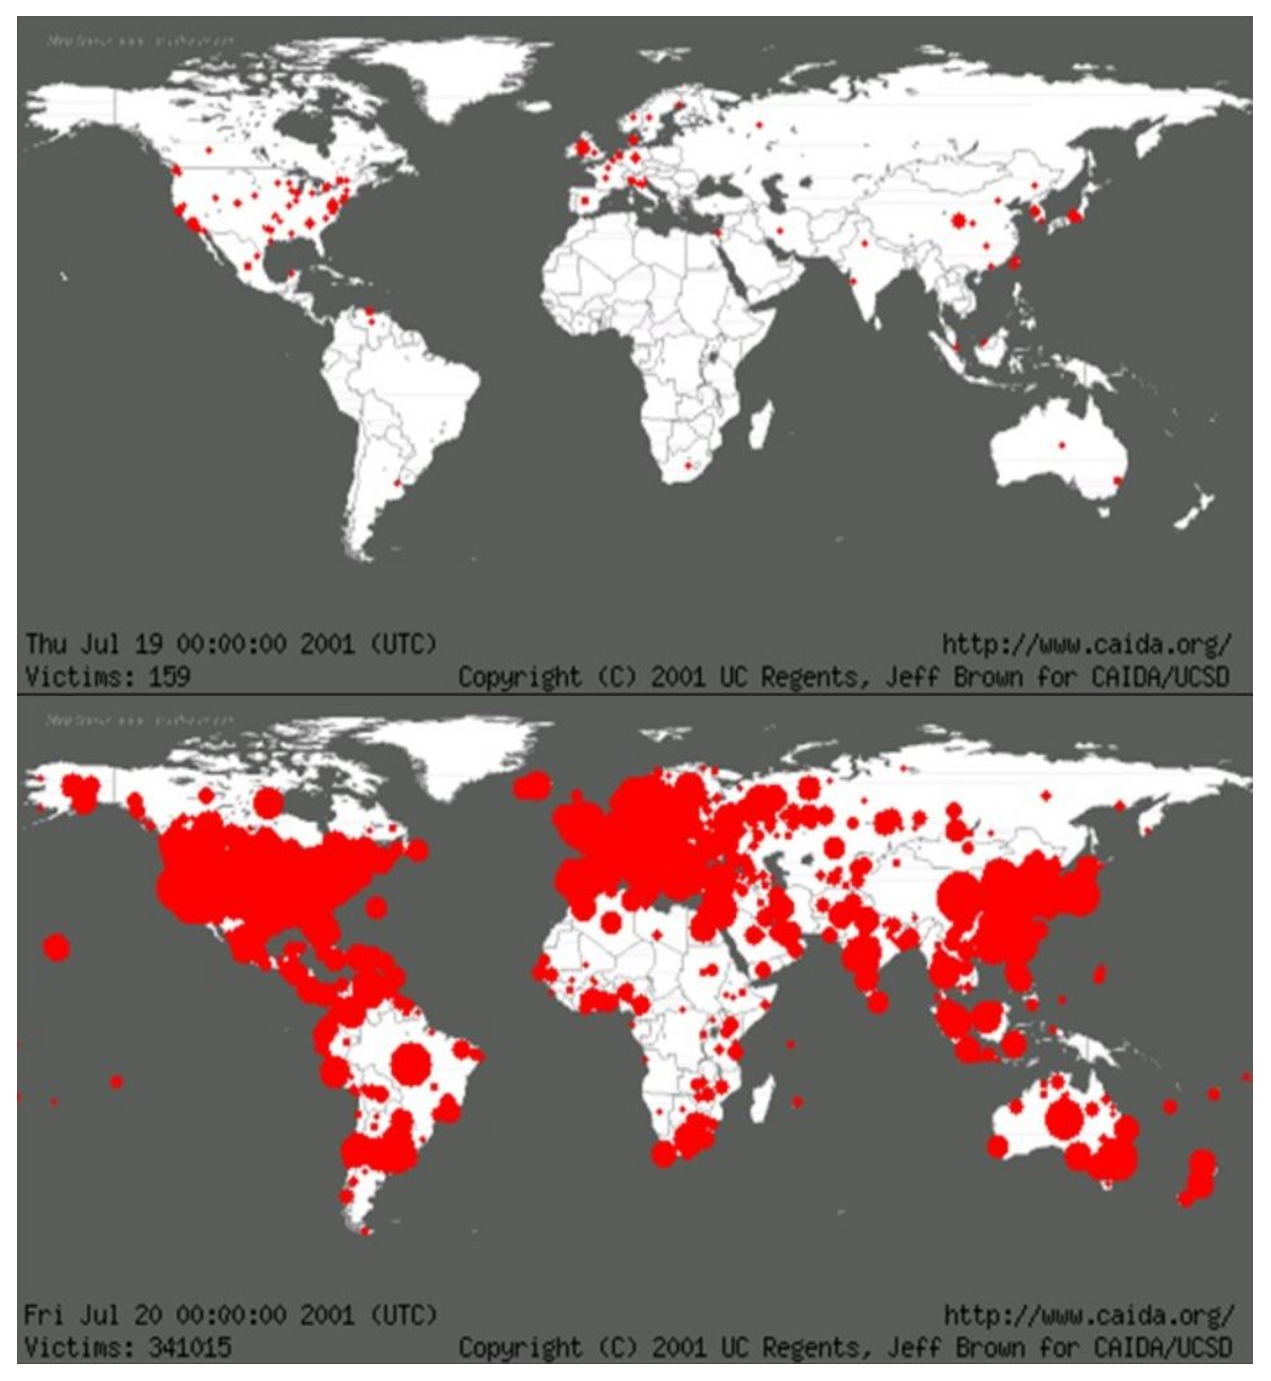
\includegraphics[width=0.8\textwidth]{images/spread.eps}
\caption{diffusione Code Red}
\label{spread}
\end{figure}
Le figure~\ref{infected} e~\ref{rate} danno un’idea del forte impatto che ha avuto la versione di Code Red a seme dinamico, infatti si vede che a partire dalla mattina del 19 Luglio c’è stato un improvviso incremento del tasso di infezione che ha raggiunto un valore di 2000 host al minuto. È interessante notare anche la decrescita esponenziale di tale tasso, dovuta probabilmente al conseguente stato di indisponibilità dei server, all’adozione di contromisure e ai gravi problemi causati alla rete globale che hanno portato ad un inevitabile rallentamento del traffico.\\
\begin{figure}
    \centering
    \begin{minipage}{0.5\textwidth}
        \centering
        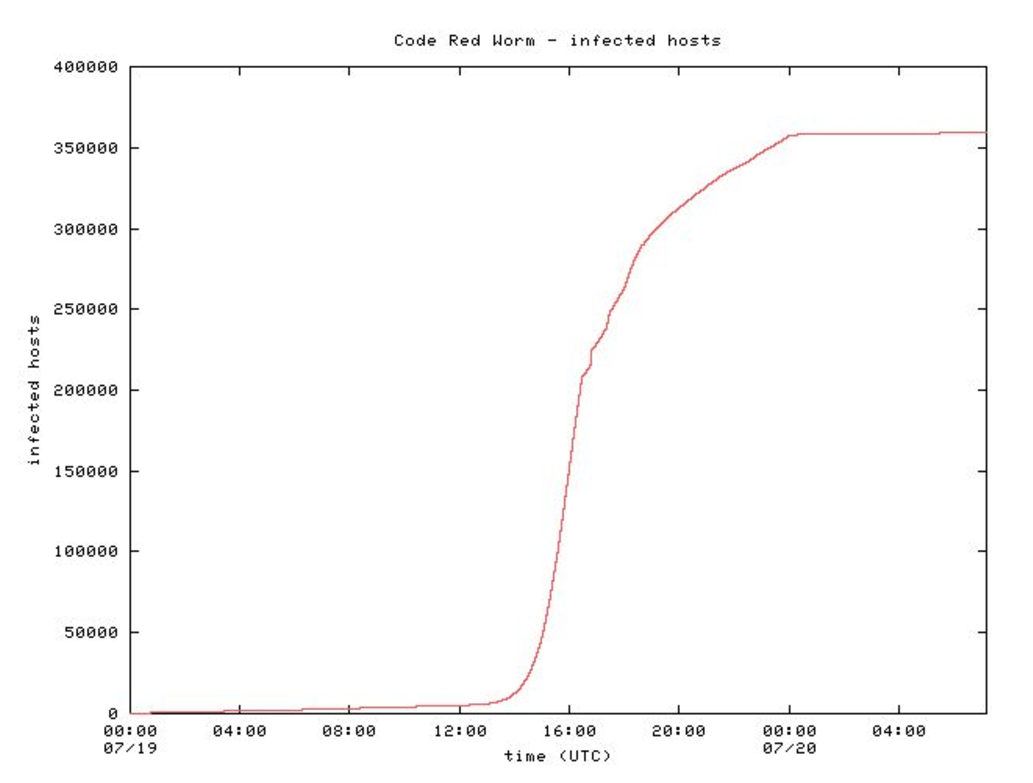
\includegraphics[width=0.95\textwidth]{images/infected} % first figure itself
        \caption{totale host infettati}
        \label{infected}
    \end{minipage}\hfill
    \begin{minipage}{0.5\textwidth}
        \centering
        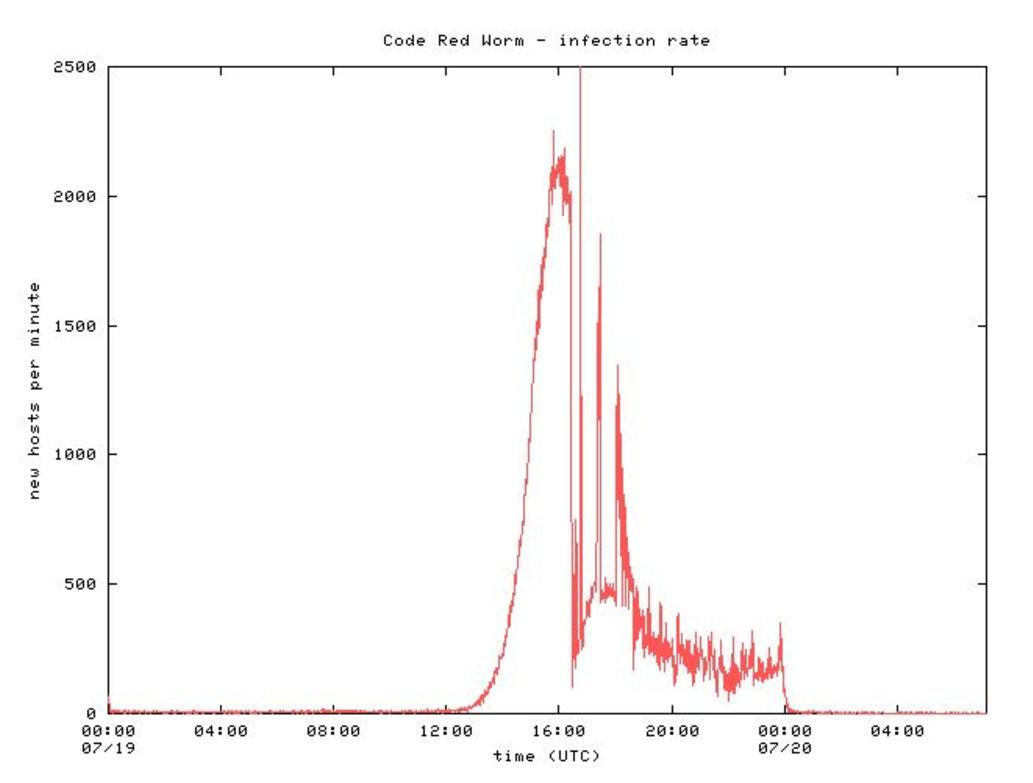
\includegraphics[width=0.95\textwidth]{images/infection_rate} % second figure itself
        \caption{tasso di infezione}
        \label{rate}
    \end{minipage}
\end{figure}
La figura ~\ref{deactivated} mostra il numero di host che hanno smesso di sondare la rete al variare del tempo e, a conferma di quanto detto sopra, tale numero era già pari a circa 200000 unità (oltre il 50\% delle infezioni totali) prima che il worm cessasse definitivamente l’attività di diffusione per procedere alla fase di attacco DDoS.\\
\begin{figure}[!hbp]
\centering
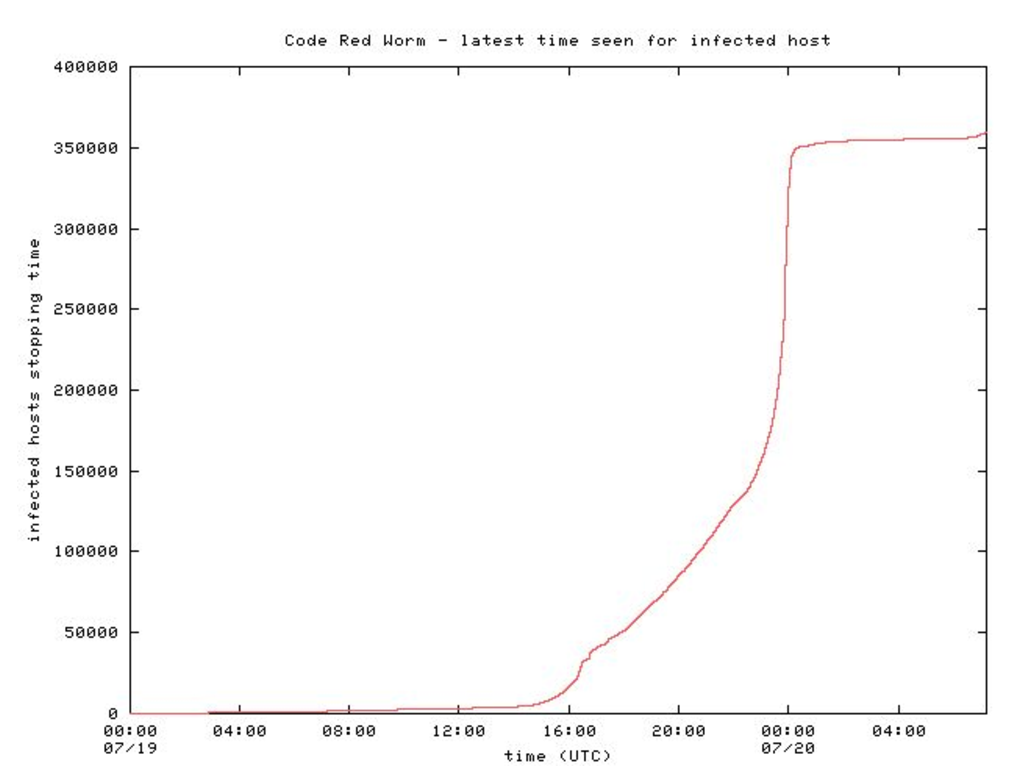
\includegraphics[width=0.7\textwidth]{images/deactivated.eps}
\caption{host "disattivati"}
\label{deactivated}
\end{figure}
Per comprendere la composizione demografica dell’utenza coinvolta, i ricercatori del CAIDA~\cite{caida} hanno esaminato i vari livelli di dominio e la locazione geografica degli host infetti.\\
La figura~\ref{domains} riassume i risultati di tale studio: per quanto riguarda i domini di primo livello la proporzione rispetta la allora attuale situazione dei web server, mentre è curioso notare che il 10\% delle macchine compromesse sono state localizzate in Korea; i principali nomi di dominio sono costituiti da server provider per infrastrutture casalinghe e piccole imprese, da qui si vede che anche queste piccole realtà hanno un ruolo rilevante riguardo la salute globale di internet.\\
\begin{figure}[!hbp]
\centering
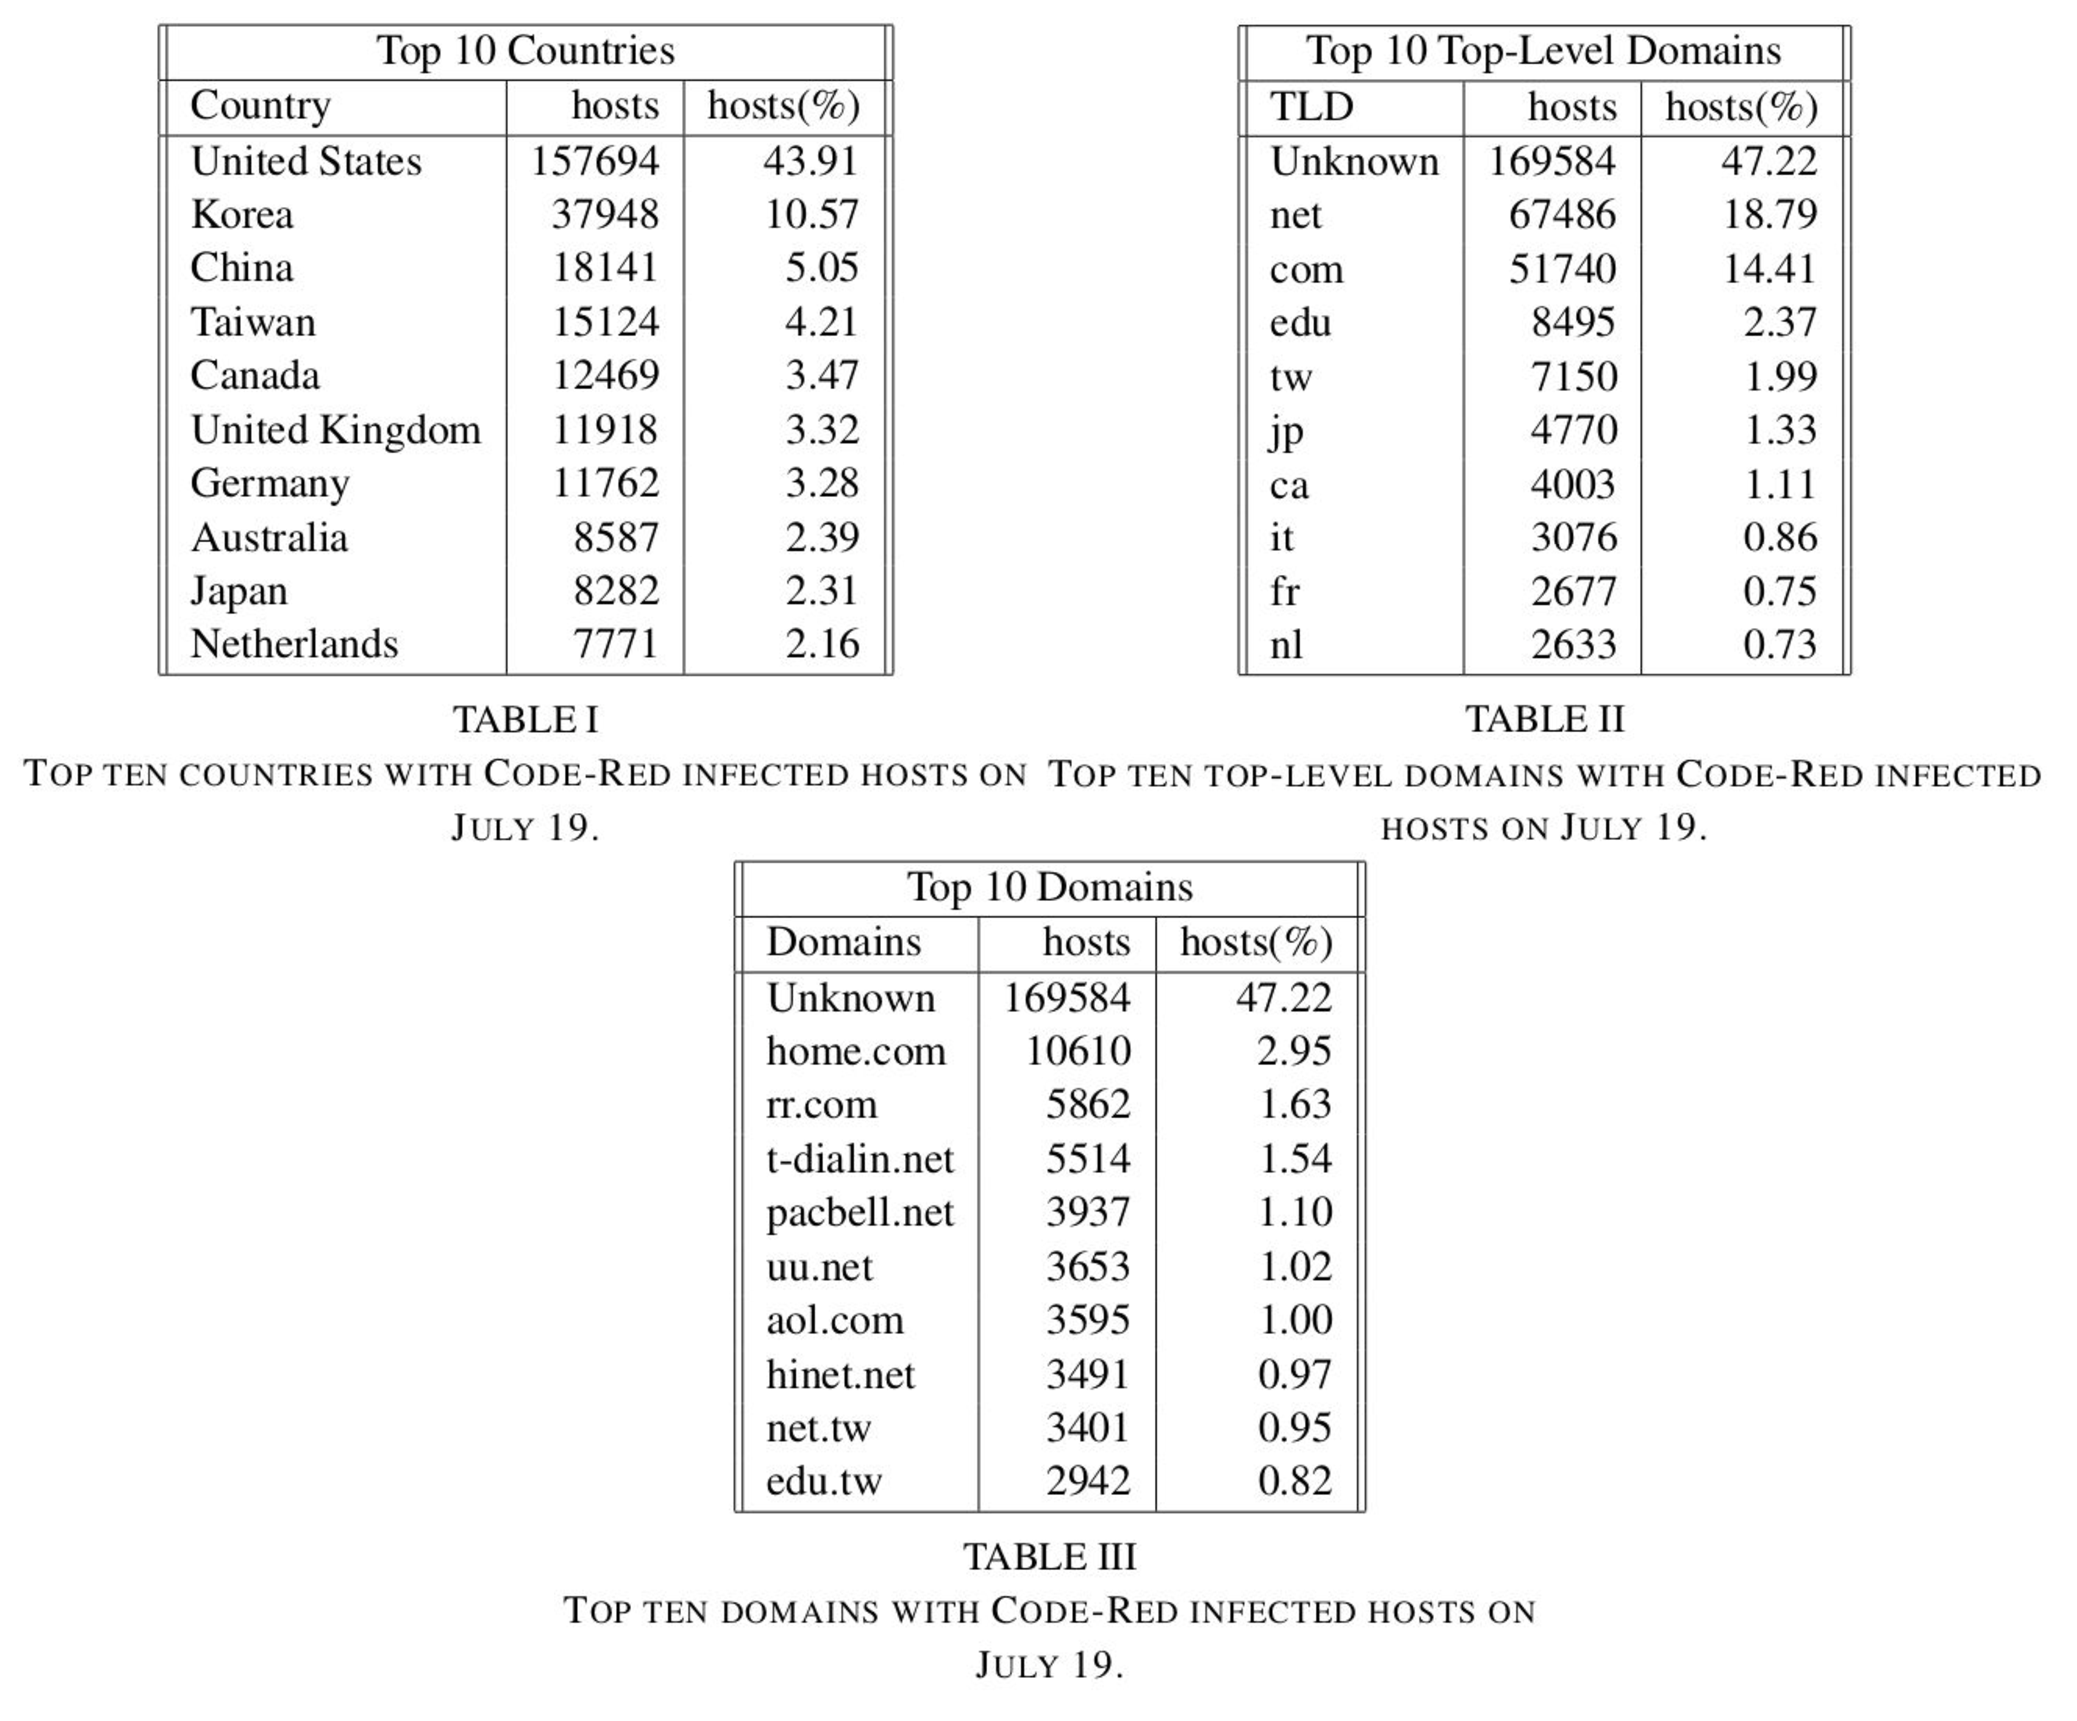
\includegraphics[width=0.8\textwidth]{images/domains.eps}
\caption{risultati analisi demografica}
\label{domains}
\end{figure}


\section{Conseguenze e impatto economico}
I principali effetti del worm Code Red furono il degradamento delle prestazioni e la perdità di stabilità dei sistemi coinvolti. Il costo globale complessivo stimato fu di 2.6 miliardi di dollari [fonti: Sans, Computereconomics] , di cui 1.1 miliardi impiegati nell’ispezione ed il recupero dei server ed i restanti 1.5 miliardi riguardarono le perdite di produttività a seguito dell’indisponibilità dei sistemi.\\
Quest’ultimi comprendevano non soltanto le macchine server degli utenti finali, ma anche vaste porzioni dell’infrastruttura di rete che furono completamente disabilitate, molte compagnie provider di dispositivi di rete sperimentarono un’indisponibiltà media di ben 36 ore [fonte Sans institute].\\
Il processo di propagazione del worm ha generato un’enorme quantità di pacchetti. Sebbene il volume di questi pacchetti era relativamente piccolo rispetto al normale traffico di rete, l’ingente quantità ha causato congestionamento e gravi problemi ad alcuni ruoter, specialmente quelli con risorse limitate. Per esempio, a causa della generazione randomica degli indirizzi IP, molti pacchetti non venivano inoltrati poiché la destinazione risultava sconosciuta, finendo così per riempire le cache ARP, esaurire la memoria e provocare il riavvio dei dispositivi [fonte-cisco].\\
La figura X mostra il costo complessivo di Code Red in relazione agli incidenti più rilevanti del periodo [fonte-computereconomics].



\section{Esperimento: se Code Red non fosse stato scoperto}
Come appena visto Code Red ha costituito una vera e propria piaga, che si è propagata in ogni angolo del pianeta e ha causato gravi danni nonostante sia stato scoperto diversi giorni prima che la seconda versione facesse la sua comparsa ed iniziasse a diffondersi in modo efficace.\\
A fronte di ciò, abbiamo effettuato una simulazione per vedere cosa sarebbe accaduto se il worm non fosse stato scoperto, e quindi avere una misura dell’entità del danno in termini di numero di host compromessi, così poi da confrontare i risultati con il caso reale in cui la consapevolezza della presenza di tale minaccia ha spinto gli utenti ad adottare contromisure come patch, firewall, antivirus e simili.\\
Per fare questo, innanzitutto è stato necessario l’ausilio di un modello epidemico che simulasse fedelmente il comportamento ed in particolare la diffusione del worm.\\
I classici modelli per lo studio dello sviluppo epidemico, però, non sono adatti a replicare il comportamento di Code Red, perché non tengono conto delle contromisure umane intraprese durante il processo di diffusione e inoltre considerano il tasso di infezione costante nel tempo. Questi due fattori hanno portato Zou et al.~\cite{two-factor} alla derivazione del “Two Factor Worm Model” con cui hanno dimostrato tramite simulazione che i risultati approssimano bene l’andamento dei dati osservati, in particolare sono riusciti a giustificare il rallentamento delle scansioni che si è verificato appena prima il cessamento dell’attività di diffusione del worm. Tale evento, infatti, è la conseguenza della violenta propagazione su larga scala che ha provocato congestionamento e danni alla rete.\\
Le figure~\ref{tf_model} e~\ref{tf_compare} mostrano i risultati ottenuti da Zou et al., in particolare la figura~\ref{tf_compare} mostra il confronto con i dati reali osservati da Goldsmith and Eichman~\cite{gold, eich}.\\
\begin{figure}
    \centering
    \begin{minipage}{0.5\textwidth}
        \centering
        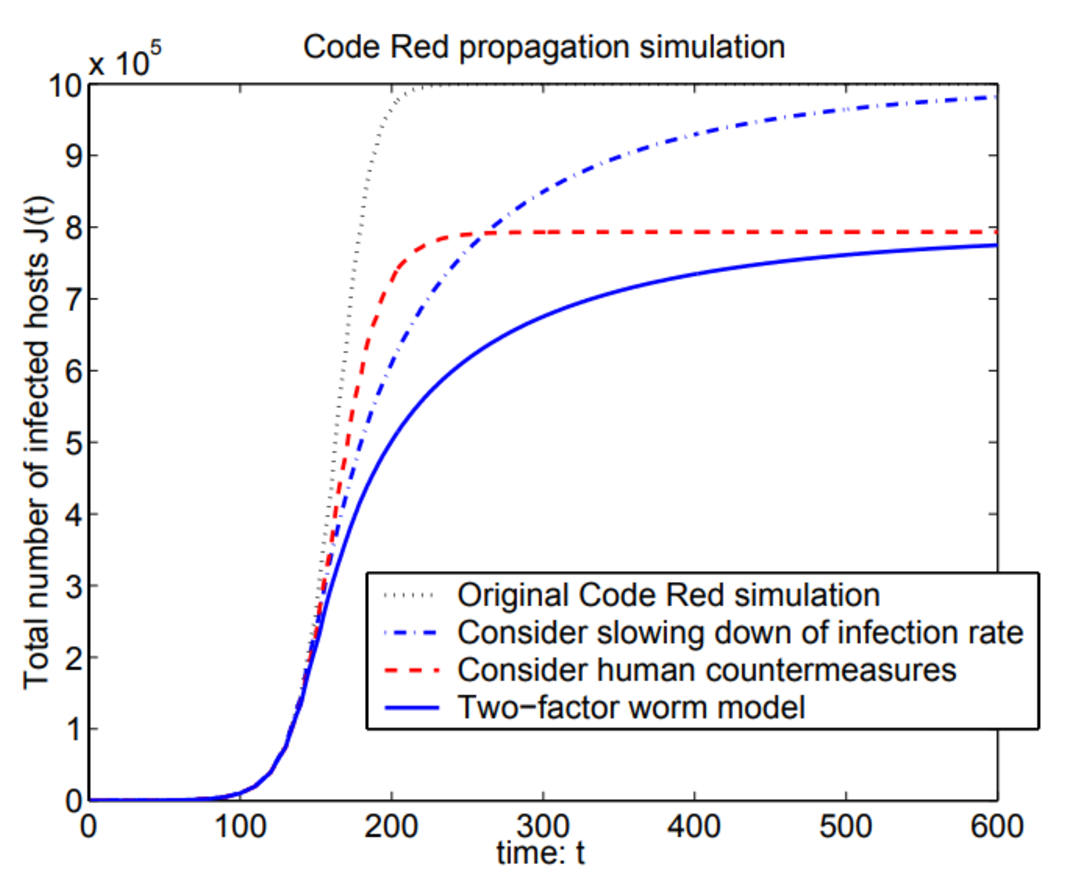
\includegraphics[width=0.95\textwidth]{images/tf_model} % first figure itself
        \caption{infezioni al variare del tempo}
        \label{tf_model}
    \end{minipage}\hfill
    \begin{minipage}{0.5\textwidth}
        \centering
        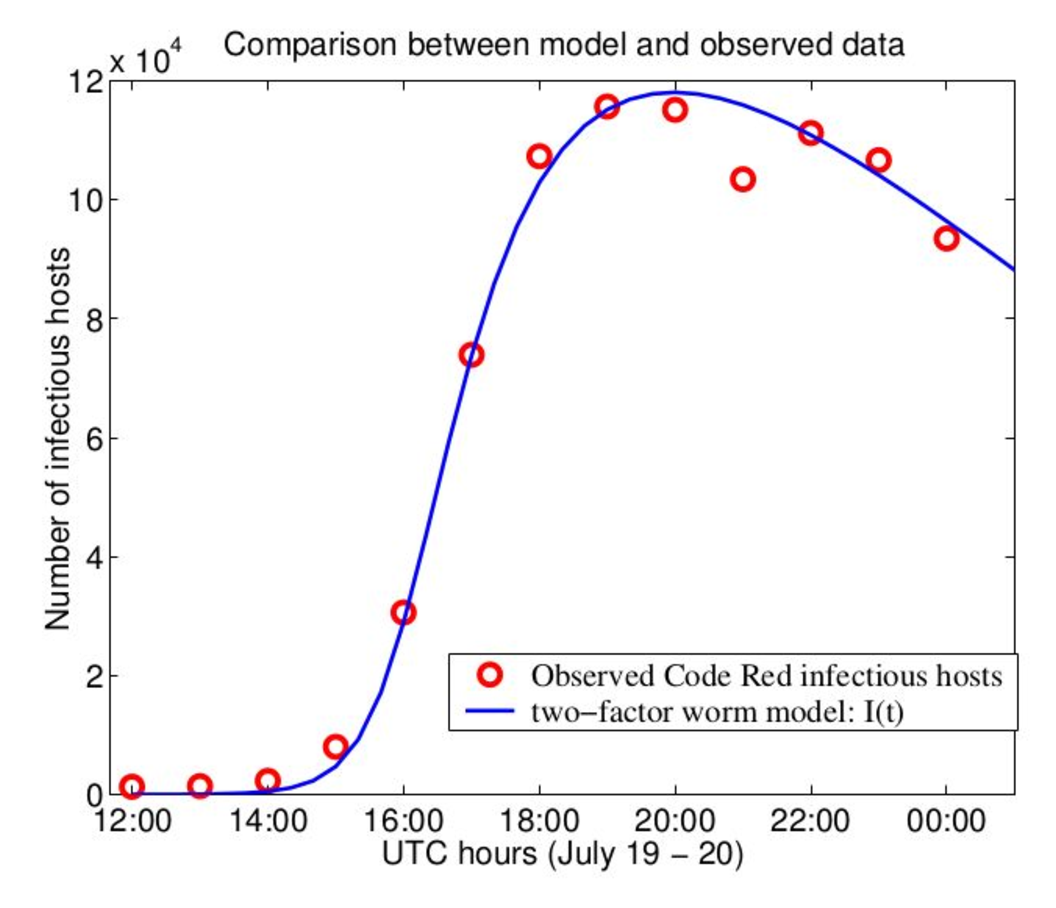
\includegraphics[width=0.95\textwidth]{images/tf_compare} % second figure itself
        \caption{confronto dati-modello}
        \label{tf_compare}
    \end{minipage}
\end{figure}
Di seguito è riportato il set di equazioni differenziali che descrivono il sistema, caratterizzanti sono il fattore $\beta(t)$ che rappresenta la frequenza di infezione variabile nel tempo, ed i fattori $R(t)$ e $Q(t)$ che costituiscono il numero di host rimossi dalla popolazione infetta a seguito di contromisure a valle del contagio, ed il numero di host rimossi dalla popolazione suscettibile (vulnerabile) a seguito di contromisure a monte, le altre variabili sono riassunte nella tabella di figura~\ref{notations}.\\
\begin{equation}
\left\{  \begin{array}{rcl} 
                dS(t)/dt &=& -\beta(t)S(t)I(t) - dQ(t)/dt, \\ 
                dR(t)/dt &=& \gamma I(t), \\ 
                dQ(t)/dt &=& \mu S(t)J(t), \\ 
                \beta(t) &=& \beta_{0}[1 - I(t)/N]^{\eta}, \\ 
                N &=& S(t) + I(t) + R(t) + Q(t), \\
                I(0) &=& I_{0} \ll N; S(0) = N -I_{0}; R(0) = Q(0) = 0; 
           \end{array}  \right.
\end{equation}
La simulazione è stata eseguita con lo stato iniziale specificato dai seguenti parametri: $N = 1000000$, $I_{0} = 1$, $\eta = 3$, $\gamma = 0.05$, $\mu = 0.06/N$ , e $\beta_{0} = 0.8/N$.\\
$I_{0}$ e $\beta_{0}$ rappresentano rispettivamente numero di host infetti e tasso di infezione iniziali, $\gamma$ e $\mu$ i tassi di rimozione, infine $\eta$ è un parametro di sensibilità che regola $\beta(t)$ in funzione di $I(t)$, sostanzialmente è un fattore che indica quanto il tasso di infezione dipende dal numero di host infetti in un certo istante di tempo, ad esempio $\eta = 0$ implica un tasso di infezione costante.\\
\begin{figure}[!hbp]
\centering
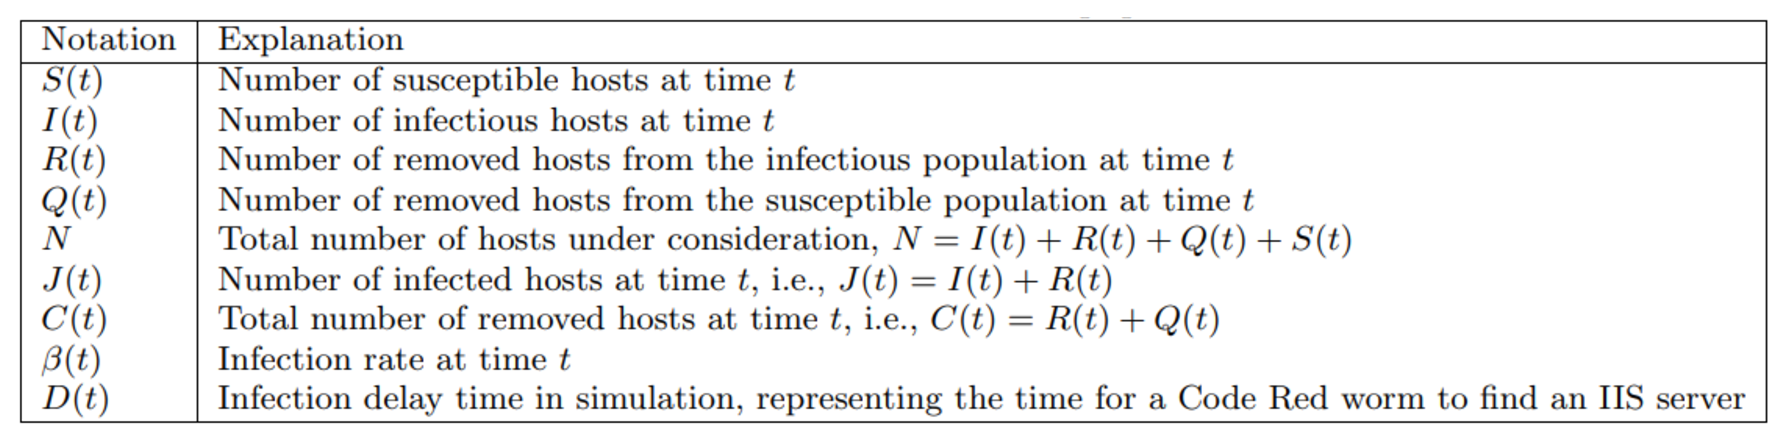
\includegraphics[width=0.95\textwidth]{images/notations.eps}
\caption{notazioni variabili del modello}
\label{notations}
\end{figure}
Il nostro studio è consistito nel semplificare il “Two Factor Model” eliminando il fattore relativo alle contromisure intraprese dagli utenti, proprio come se il worm avesse potuto agire indisturbato senza che nessuno si accorgesse della sua presenza, pertanto le variabili  R(t) e Q(t) relative agli host in stato di “rimosso” sono state annullate, ottenendo così il seguente modello semplificato:
\begin{equation}
\left\{  \begin{array}{rcl} 
                dS(t)/dt &=& -\beta(t)S(t)I(t), \\ 
                \beta(t) &=& \beta_{0}[1 - I(t)/N]^{\eta}, \\ 
                N &=& S(t) + I(t), \\
                I(0) &=& I_{0} \ll N; S(0) = N -I_{0}; 
           \end{array}  \right.
\end{equation}
La simulazione è stata realizzata tramite Simulink, a partire dalle stesse condizioni iniziali poste da Zou et al. e per un tempo di simulazione equivalente a circa 24h.\\
I risultati ottenuti (Figura~\ref{simpler}) mostrano che in 12 ore (metà tempo di simulazione) circa il 70\% degli host suscettibili sono stati infettati, approssimativamente la stessa proporzione della simulazione effettuata da Zou et al., quindi in definitiva il fatto che Code Red sia stato scoperto prima della sua violenta diffusione non ha alleviato significativamente le conseguenze in termini di macchine infettate.\\
Questo risultato mette in evidenza che di fronte ad un worm così aggressivo come Code Red, con un tasso di propagazione che ha raggiunto un picco di 2000 infezioni al minuto, le contromisure che vengono adottate a seguito dell’inizio dell’epidemia non contribuiscono a porre rimedio in maniera efficace da un punto di vista globale, ma ciò che può fare la differenza sono le contromisure preventive che vengono attuate prima degli attacchi, ovvero quelle che tendono a ridurre il numero di host potenzialmente a rischio. Quindi il vero fattore che ha favorito gli effetti devastanti del worm è stata la mancata applicazione della patch che andava ad eliminare la vulnerabilità sfruttata, nonostante fosse stata resa disponibile non poche settimane prima della comparsa della minaccia.\\
\begin{figure}[!h]
\centering
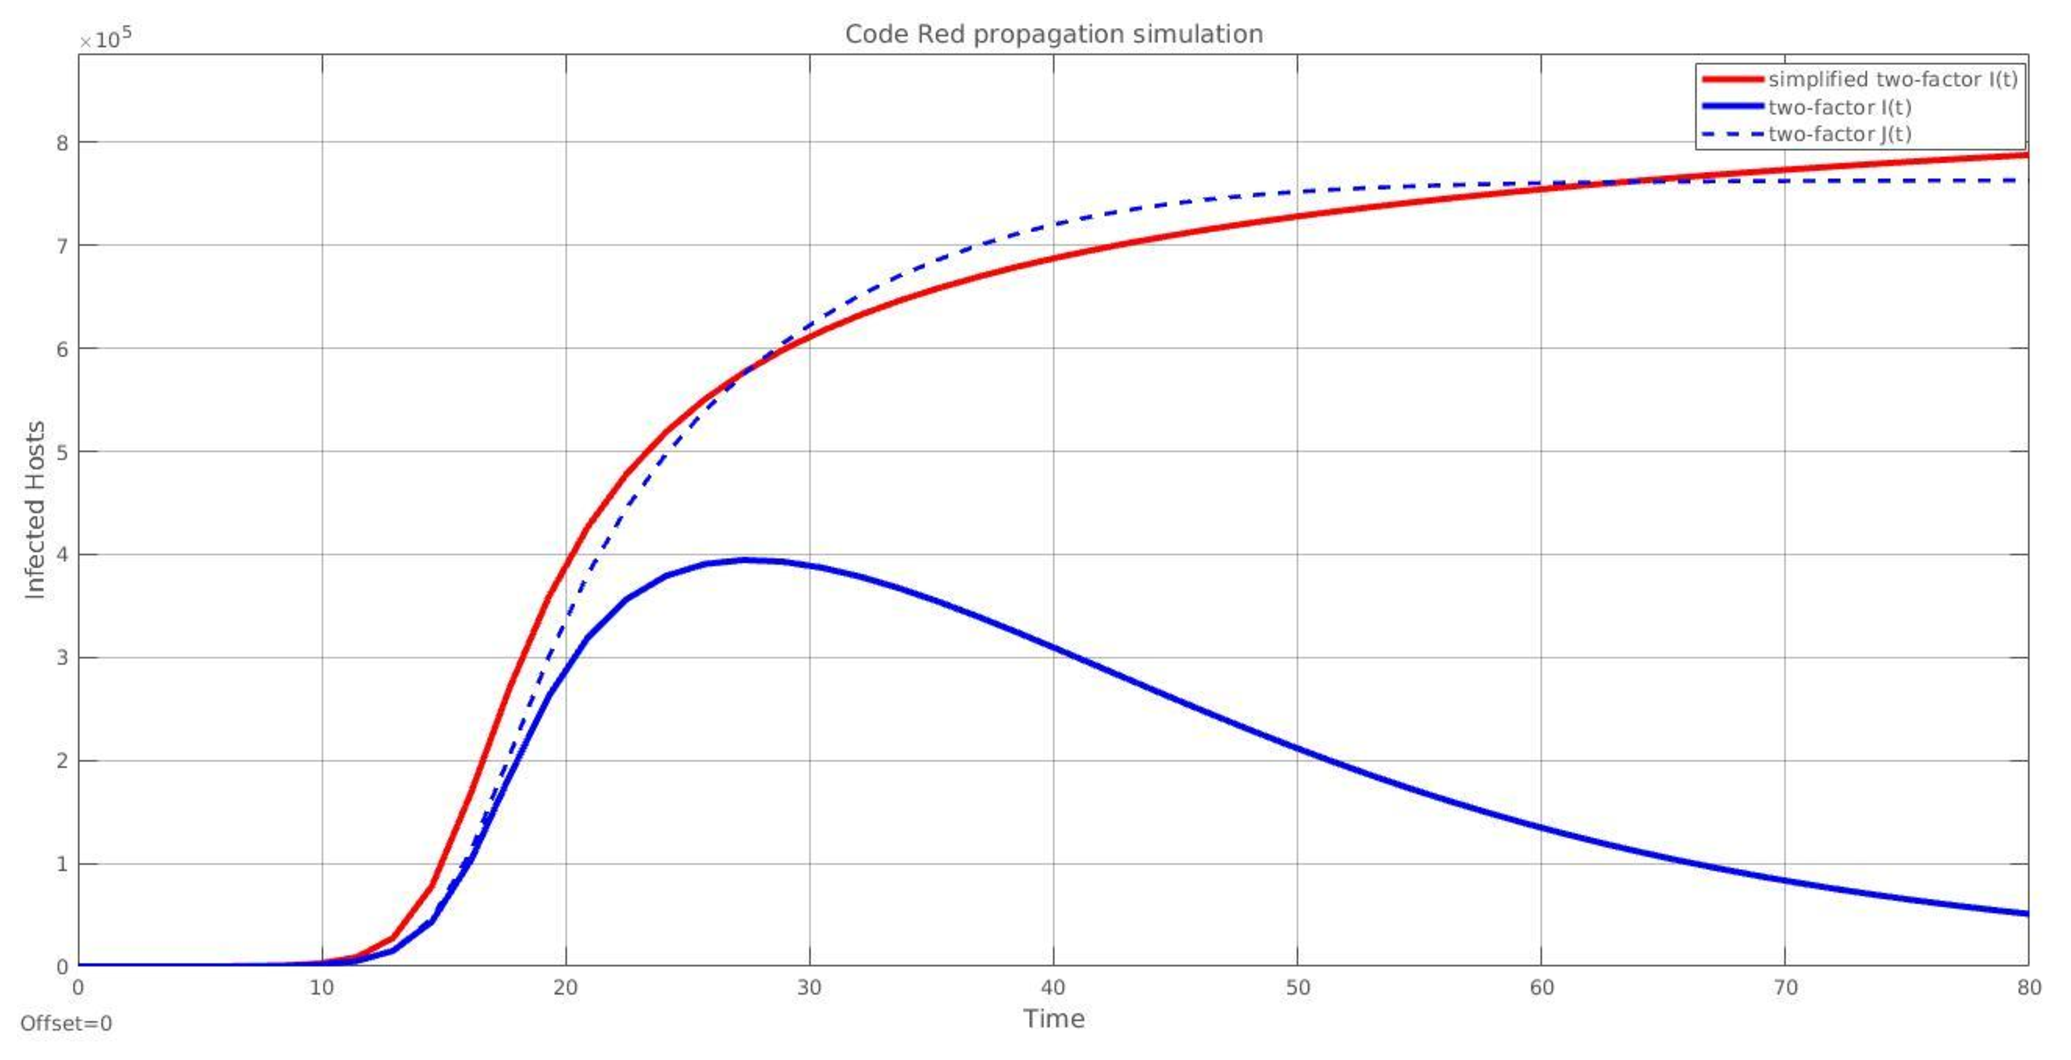
\includegraphics[width=0.95\textwidth]{images/simpler.eps}
\caption{modello semplificato vs. two-factor}
\label{simpler}
\end{figure}


\section{Contromisure}

\section{Conclusioni}

\newpage
\begin{thebibliography}{99}

\bibitem{eeye} 
\emph{``ANALYSIS: .ida "Code Red" Worm''}
eEye. July 17, 2001\\
\url{https://web.archive.org/web/20110722192419/http://www.eeye.com/Resources/Security-Center/Research/Security-Advisories/AL20010717}

\bibitem{bullet}
\emph{``Microsoft Security Bulletin MS01-033 - Critical''}
Microsoft. June 18, 2001\\
\url{https://docs.microsoft.com/en-us/security-updates/securitybulletins/2001/ms01-033}

\bibitem{caida} Moore, David \& Shannon, Colleen \& Brown, Jeffery. 
\emph{``Code-Red: a case study on the spread and victims of an Internet worm''}
CAIDA.\\
\url{http://www.caida.org/publications/papers/2002/codered/codered.pdf}

\bibitem{two-factor} Cliff Changchun Zou, Weibo Gong, Don Towsley.
\emph{``Code Red Worm Propagation Modeling and Analysis.''}
Dept. Electrical \& Computer Engineering Univ. Massachusetts Amherst, MA\\
\url{http://www.cs.ucf.edu/~czou/research/codered.pdf}

\bibitem{selke} Sarah Sellke, Ness B. Shroff, and Saurabh Bagchi.
\emph{``Modeling and Automated Containment of Worms.''}
School of Electrical and Computer Engineering Purdue University\\
\url{https://ieeexplore.ieee.org/document/4358715/}

\bibitem{ce}
\emph{``Malicious Code Attacks Had \$13.2 Billion Economic Impact in 2001.''}
Computer Economics. September, 2002\\
\url{https://www.computereconomics.com/article.cfm?id=133}

\bibitem{sans} Schauer, Renee C..
\emph{``The Mechanisms and Effects of the Code Red Worm.''}
Sans Institute. 2001\\
\url{https://www.sans.org/reading-room/whitepapers/dlp/the-mechanisms-and-effects-of-the-code-red-worm-87}

\bibitem{cisco}
\emph{``Code Red Worm - Customer Impact.''}
Cisco. July 20, 2001\\
\url{https://tools.cisco.com/security/center/content/CiscoSecurityAdvisory/cisco-sa-20010720-code-red-worm}

\bibitem{eich} K. Eichman.
\emph{``Possible CodeRed Connection Attempts.''}
July 20, 2001\\
\url{http://lists.jammed.com/incidents/2001/07/0159.html}

\bibitem{gold} D. Goldsmith. 
\emph{``Possible CodeRed Connection Attempts.''}
July 20, 2001\\
\url{http://lists.jammed.com/incidents/2001/07/0149.html}

\bibitem{sans-acl} Dennis Eck.
\emph{``Access Control Lists to Protect a Network from Worm/DoS Attacks.''}
Sans Institute. December 4, 2003\\
\url{https://www.giac.org/paper/gsec/3551/access-control-lists-protect-network-worm-dos-attacks/105776}

\bibitem{sans-acl} William Geige.
\emph{``Proactively Guarding Against Unknown Web Server Attacks.''}
Sans Institute.\\
https://www.giac.org/paper/gsec/1153/proactively-guarding-unknown-web-server-attacks/102250
\end{thebibliography}

\end{document}
